\hypertarget{distributed-memory-systems-and-message-passing-interface-mpi}{%
\section{Distributed Memory Systems and Message Passing Interface
(MPI)}\label{distributed-memory-systems-and-message-passing-interface-mpi}}

\hypertarget{shared--vs.distributed-memory-systems}{%
\subsection{Shared- vs.~Distributed Memory
Systems}\label{shared--vs.distributed-memory-systems}}

\begin{itemize}
\tightlist
\item
  Not all MIMD (multiple input multiple data) systems can be
  shared-memory systems

  \begin{itemize}
  \tightlist
  \item
    the cost of scaling of interconnect is very high
  \item
    distributed-memory interconnects such as the hypercube and the
    toroidal mesh are relatively inexpensive
  \item
    distributed-memory systems are often better suited for problems
    requiring vast amounts of data or computation
  \end{itemize}
\item
  Shared-memory systems carry out their tasks by \textbf{threads}
\item
  Distributed-memory systems carry out their tasks by
  \textbf{processess}

  \begin{itemize}
  \tightlist
  \item
    processes have their own address space and can communicate to each
    other by different concepts: message passing, pipes, remotely
    shared- memory, \ldots{}
  \end{itemize}
\end{itemize}

\hypertarget{motivation-map-reduce}{%
\subsubsection{Motivation Map-Reduce}\label{motivation-map-reduce}}

\begin{figure}[H]
\centering
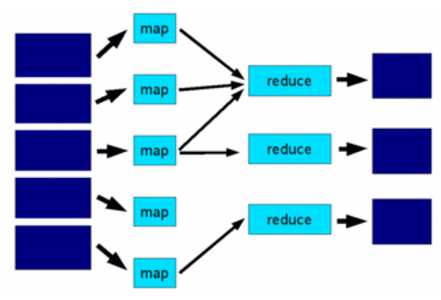
\includegraphics[width=0.5\textwidth]{figures/mapreduce.png}
\caption{Map-Reduce}
\end{figure}

\begin{figure}[H]
\centering
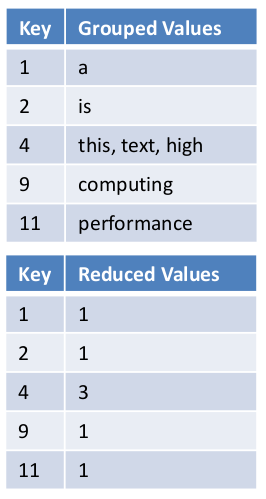
\includegraphics[width=0.3\textwidth]{figures/maprecudeExample.png}
\caption{Map-Reduce Example}
\end{figure}

\begin{itemize}
\tightlist
\item
  map

  \begin{itemize}
  \tightlist
  \item
    a stream of input data is mapped into several groups on basis of a
    function
  \item
    map returns for each item a map \textless{}key, value\textgreater{}
  \item
    it groups all return values by the keys
  \item
    In our example, the groups could then be distributed to several
    nodes then
  \end{itemize}
\item
  reduce

  \begin{itemize}
  \tightlist
  \item
    takes a key and all values associated with that key and computes a
    reduction result of all associated values
  \item
    reduction can be computed in parallel for all keys
  \end{itemize}
\item
  example

  \begin{itemize}
  \tightlist
  \item
    input: ``this is a text high performance computing''
  \end{itemize}
\end{itemize}

\clearpage
\hypertarget{message-passing-interface-mpi}{%
\subsection{Message Passing Interface
(MPI)}\label{message-passing-interface-mpi}}

MPI is a standardized and portable message-passing system to function on
a wide variety of parallel computing architectures.

\begin{itemize}
\tightlist
\item
  Ein Node ist Host, der verschiedene Prozesse betreiben kann
\item
  In MPI spricht man nicht von Prozess 2, sondern von Rank 2
\item
  Das Programm muss vorgängig auf jedem Node verfügbar sein
\end{itemize}

\begin{figure}[H]
\centering
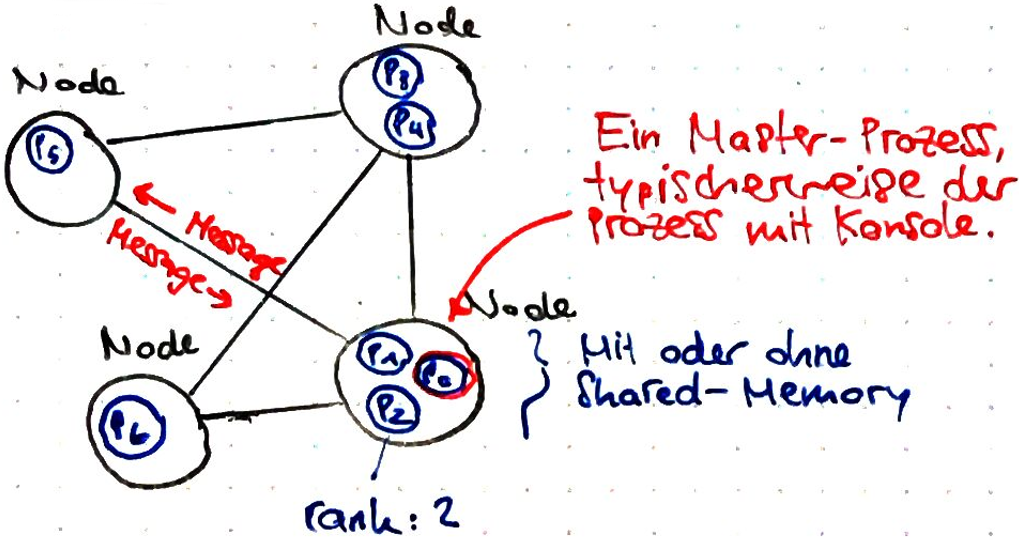
\includegraphics[width=0.5\textwidth]{figures/mpi_idea.png}
\caption{MPI Idea}
\end{figure}

\begin{itemize}
\tightlist
\item
  a machine consists of p processes, each with its own exclusive address
  space
\item
  asynchronous paradigm

  \begin{itemize}
  \tightlist
  \item
    all concurrent tasks execute asynchronously
  \end{itemize}
\item
  loosely synchronous model

  \begin{itemize}
  \tightlist
  \item
    tasks or subsets of tasks synchronize to perform interactions
  \item
    between these interactions, tasks execute completely asynchronously
  \end{itemize}
\item
  SPMD model

  \begin{itemize}
  \tightlist
  \item
    most message-passing programs are written using the Single Program
    Multiple Data model
  \end{itemize}
\end{itemize}

\clearpage
\hypertarget{simple-mpi-example}{%
\subsubsection{Simple MPI Example}\label{simple-mpi-example}}

The implementation can be in C or in C++.

\begin{lstlisting}[language=C++]
// #include <mpi.h> <iostream> <sstream> using namespace std;

int main(int argc, char* argv[]) {
    int numprocs, myid;

    MPI_Init(&argc, &argv);
    MPI_Comm_size(MPI_COMM_WORLD, &numprocs);
    MPI_Comm_rank(MPI_COMM_WORLD, &myid);

    if (myid == 0) {
        const int bufLen = 100; char greeting[bufLen];
        cout << "Greetings from process " << myid << " of " << numprocs << " processes!" << endl;
        for (int i = 1; i < numprocs; i++) {  //I get the messages exactly in the order in which I want here (from i = 1 to numprocs)
            MPI_Recv(greeting, bufLen, MPI_CHAR, i, 0, MPI_COMM_WORLD, MPI_STATUS_IGNORE);  //In this case, MPI_Recv is blocking. There are also non-blocking implementations
            cout << greeting << endl;
        }
    } else {
        stringstream ss;
        ss << "Greetings from process " << myid << " of " << numprocs << " processes!";
        string greeting(ss.str());
        MPI_Send(greeting.c_str(), (int)greeting.size() + 1, MPI_CHAR, 0, 0, MPI_COMM_WORLD);
    }
    MPI_Finalize();
    return 0;
}

//Executing the program in VC++
//Command: $(MSMPI_BIN)mpiexec.exe
//Arguments: -n 10 "$(TargetPath)"
\end{lstlisting}

\hypertarget{set-of-mpi-routines}{%
\subsubsection{Set of MPI Routines}\label{set-of-mpi-routines}}

\begin{itemize}
\tightlist
\item
  MPI\_Init

  \begin{itemize}
  \tightlist
  \item
    initializes MPI
  \end{itemize}
\item
  MPI\_Finalize

  \begin{itemize}
  \tightlist
  \item
    terminates MPI
  \end{itemize}
\item
  MPI\_Comm\_size

  \begin{itemize}
  \tightlist
  \item
    determines the number of processes
  \end{itemize}
\item
  MPI\_Comm\_rank

  \begin{itemize}
  \tightlist
  \item
    determines the label of calling process
  \end{itemize}
\item
  MPI\_Send

  \begin{itemize}
  \tightlist
  \item
    sends a message
  \end{itemize}
\item
  MPI\_Recv receives a message
\end{itemize}

\hypertarget{how-to-debug-mpi-programs}{%
\subsubsection{How to Debug MPI
Programs?}\label{how-to-debug-mpi-programs}}

\begin{itemize}
\tightlist
\item
  Error Detection Strategies

  \begin{itemize}
  \tightlist
  \item
    run program with just one or only two processes
  \item
    run all processes on a single computer
  \item
    use assertions
  \item
    use synchronous instead of buffered communication
  \end{itemize}
\item
  Debugging

  \begin{itemize}
  \tightlist
  \item
    mpiexec.exe starts several processes and each process runs the same
    MPI program
  \item
    how to attach a debugger to one of these processes, let's say p

    \begin{itemize}
    \tightlist
    \item
      use GetCurrentProcessId() or getpid() to determine the process ID
      of p
    \item
      block process p by using stdin or MPI\_Recv to attach the debugger
    \item
      set your breakpoints and release process p
    \end{itemize}
  \end{itemize}
\end{itemize}

\hypertarget{semantics-of-point-to-point-communication}{%
\subsection{Semantics of Point-to-Point
Communication}\label{semantics-of-point-to-point-communication}}

\hypertarget{send-and-receive-operations}{%
\subsubsection{Send and Receive
Operations}\label{send-and-receive-operations}}

\begin{figure}[H]
\centering
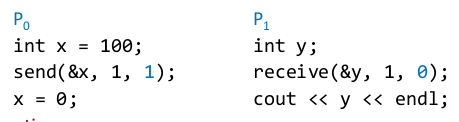
\includegraphics[width=0.6\textwidth]{figures/sendReceiveMPI.png}
\caption{Send and Receive Operations}
\end{figure}

In the above example it is important, that x is not changed until send
of x is successfully executed. If send would be blocking, this is not
dangerous.

\hypertarget{blocking-message-passing-operations}{%
\subsubsection{Blocking Message Passing
Operations}\label{blocking-message-passing-operations}}

\begin{itemize}
\tightlist
\item
  Non-Buffered

  \begin{itemize}
  \tightlist
  \item
    in the non-buffered blocking send, the operation does not return
    until the matching receive has been encountered at the receiving
    process
  \item
    idling and deadlocks are major issues with non-buffered blocking
    sends
  \end{itemize}
\end{itemize}

\begin{figure}[H]
\centering
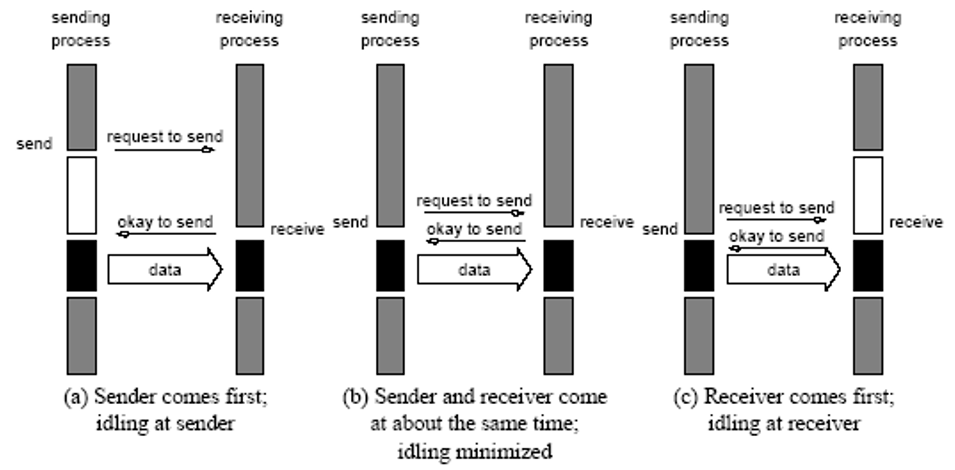
\includegraphics[width=0.9\textwidth]{figures/BlockingNonBufferMPI.png}
\caption{Blocking Non Buffer MPI}
\end{figure}

\begin{itemize}
\tightlist
\item
  Buffered

  \begin{itemize}
  \tightlist
  \item
    a simple solution to the idling and deadlocking problem outlined
    before is to rely on buffers at the sending and receiving ends
  \item
    the sender copies the data into the designated buffer and returns
    after copying has been completed; the data must be buffered at the
    receiving end as well
  \item
    buffering trades off idling overhead for buffer copying overhead
  \item
    The left side of the example is with DMA, the right one without.
  \end{itemize}
\end{itemize}

\begin{figure}[H]
\centering
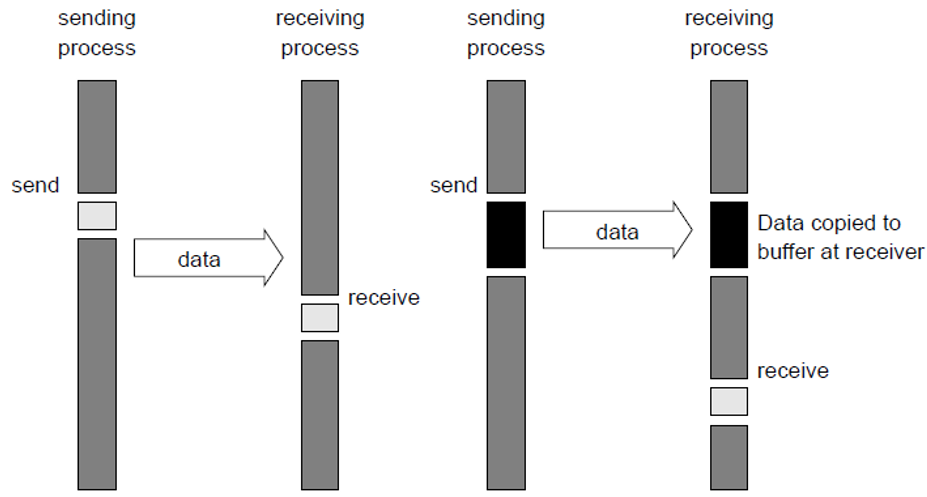
\includegraphics[width=0.7\textwidth]{figures/blockingBufferMPI.png}
\caption{Blocking Buffer MPI}
\end{figure}

\hypertarget{blocking-routine}{%
\subsubsection{Blocking Routine}\label{blocking-routine}}

\begin{lstlisting}[language=C++]
int MPI_Send(void *buf, int count, MPI_Datatype datatype, int dest,
    int tag, MPI_Comm comm)
int MPI_Recv(void *buf, int count, MPI_Datatype datatype, int source,
    int tag, MPI_Comm comm, MPI_Status *status)
\end{lstlisting}

\begin{itemize}
\tightlist
\item
  MPI\_Datatypes

  \begin{itemize}
  \tightlist
  \item
    MPI provides equivalent datatypes for all C datatypes
  \item
    e.g.~MPI\_BYTE corresponds to a byte (8 bits) and MPI\_PACKED
    corresponds to a collection of data items that has been created by
    packing non-contiguous data
  \end{itemize}
\item
  Destination and Source

  \begin{itemize}
  \tightlist
  \item
    destination and source processes are uniquely defined by process ID
    (= rank) and communicator (process subset)
  \item
    source wildcard in MPI\_Recv: MPI\_ANY\_SOURCE
  \item
    no destination in MPI\_Send: MPI\_PROC\_NULL
  \end{itemize}
\item
  Tag

  \begin{itemize}
  \tightlist
  \item
    user defined message-tag to distinguish different types of messages
  \item
    tag wildcard: MPI\_ANY\_TAG
  \end{itemize}
\end{itemize}

\hypertarget{safety-and-deadlocks}{%
\subsubsection{Safety and Deadlocks}\label{safety-and-deadlocks}}

\begin{lstlisting}[language=C++]
int a[10], b[10], myid;
MPI_Status status;
...
MPI_Comm_rank(MPI_COMM_WORLD, &myid);
if (myid == 0) {
    const int dest = 1;
    MPI_Send(a, 10, MPI_INT, dest, 1, MPI_COMM_WORLD);
    MPI_Send(b, 10, MPI_INT, dest, 2, MPI_COMM_WORLD);
} else if (myid == 1) {
    const int source = 0;
    MPI_Recv(b, 10, MPI_INT, source, 2, MPI_COMM_WORLD, &status);
    MPI_Recv(a, 10, MPI_INT, source, 1, MPI_COMM_WORLD, &status);
}
\end{lstlisting}

This program would lead to a deadlock, since the receiver is waiting for
the message with the tag `2' and the sender is first sending the message
with the tag `1'. This happens only if the implementation is using
non-buffered MPI\_Send. But since we don't know if the implemenation is
using a buffer or not (this is implementation depending), we need to
ensure that the program is able to run correctly regardless of the two
implementations.

\clearpage
\hypertarget{ssend}{%
\subsubsection{SSend}\label{ssend}}

\begin{itemize}
\tightlist
\item
  we can use an alternative to MPI\_Send: MPI\_Ssend
\item
  synchronous sending is guaranteed to block until the matching receive
  starts, independent if the implementation is using a buffer or not.
\end{itemize}

\hypertarget{mpi_sendrecv}{%
\subsubsection{MPI\_Sendrecv}\label{mpi_sendrecv}}

sending and receiving messages simultaneously:

\begin{lstlisting}[language=C++]
int MPI_Sendrecv(void *sendbuf, int sendcount, MPI_Datatype senddatatype, int dest, int sendtag, void *recvbuf, int recvcount, MPI_Datatype recvdatatype, int source, int recvtag, MPI_Comm comm, MPI_Status *status)
\end{lstlisting}

or with same buffer for both sending and receiving:

\begin{lstlisting}[language=C++]
int MPI_Sendrecv_replace(void *buf, int count, MPI_Datatype datatype, int dest, int sendtag, int source, int recvtag, MPI_Comm comm, MPI_Status *status)
\end{lstlisting}

\hypertarget{non-blocking-message-passing}{%
\subsubsection{Non-Blocking Message
Passing}\label{non-blocking-message-passing}}

\begin{itemize}
\tightlist
\item
  the programmer must ensure semantics of the send and receive
\item
  this class of non-blocking protocols returns from the send or receive
  operation before it is semantically safe to do so
\item
  non-blocking operations are generally accompanied by a check-status
  operation
\item
  when used correctly, these primitives are capable of overlapping
  communication overheads with useful computations
\end{itemize}

\begin{figure}[H]
\centering
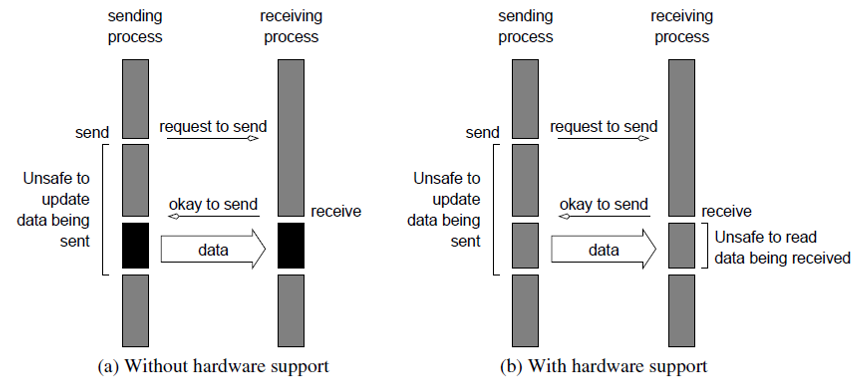
\includegraphics[width=0.8\textwidth]{figures/non-blockingSendMPI.png}
\caption{Non Blocking Send MPI}
\end{figure}

\begin{lstlisting}[language=C++]
int MPI_Isend(void *buf, int count, MPI_Datatype datatype, int dest, int tag, MPI_Comm comm, MPI_Request *request)

int MPI_Irecv(void *buf, int count, MPI_Datatype datatype, int source, int tag, MPI_Comm comm, MPI_Request *request)
\end{lstlisting}

tests whether or not the non-blocking send or receive operation
identified by its request has finished:

\begin{lstlisting}[language=C++]
int MPI_Test(MPI_Request *request, int *flag, MPI_Status *status)
\end{lstlisting}

waits for the operation to complete:

\begin{lstlisting}[language=C++]
int MPI_Wait(MPI_Request *request, MPI_Status *status)
\end{lstlisting}

\hypertarget{communication-status}{%
\subsubsection{Communication Status}\label{communication-status}}

MPI\_Status:

\begin{lstlisting}[language=C++]
struct MPI_Status {
    int MPI_SOURCE;
    INT MPI_TAG;
    INT MPI_ERROR;
};
\end{lstlisting}

MPI\_Get\_count returns the precise count of data items received:

\begin{lstlisting}[language=C++]
int MPI_Get_count(MPI_Status *status    /* in */,
MPI_Datatype datatype   /* in */,
int *count  /* out */)
\end{lstlisting}

\clearpage
\hypertarget{odd-even-sort}{%
\subsection{Odd-Even-Sort}\label{odd-even-sort}}

\begin{figure}[H]
\centering
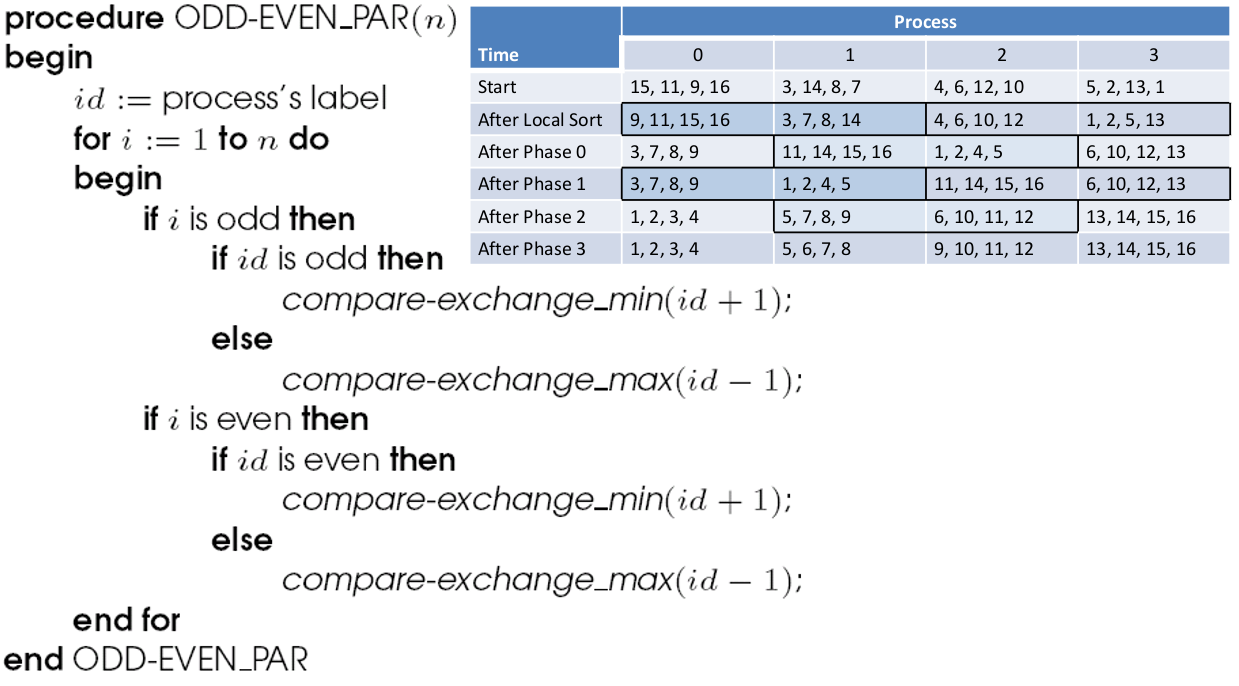
\includegraphics[width=0.8\textwidth]{figures/oddevensortMPI.png}
\caption{Parallel Odd-Even Sort}
\end{figure}

\begin{figure}[H]
\centering
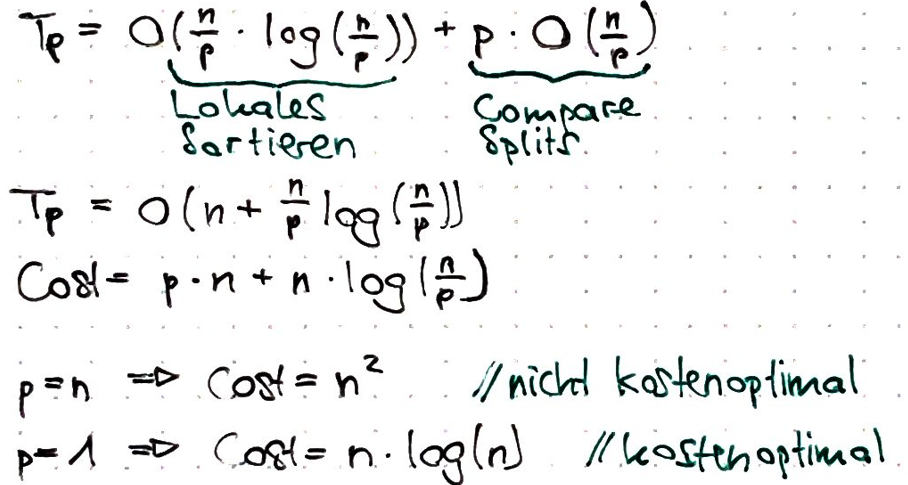
\includegraphics[width=0.6\textwidth]{figures/laufzeitberechnung-Odd-Even-Sort.png}
\caption{Laufzeitberechnung Odd-Even Sort}
\end{figure}

\clearpage
\hypertarget{communicators-and-topologies}{%
\subsection{Communicators and
Topologies}\label{communicators-and-topologies}}

\hypertarget{communication-domain}{%
\subsubsection{Communication Domain}\label{communication-domain}}

\begin{itemize}
\tightlist
\item
  Communication Domain

  \begin{itemize}
  \tightlist
  \item
    a communicator defines \textbf{a set of processes} that are allowed
    to communicate with each other (intra-communication)
  \item
    information about communication domains is stored in variables of
    type MPI\_Comm
  \item
    a process can belong to many different (possibly overlapping)
    communication domains
  \end{itemize}
\item
  Communicators

  \begin{itemize}
  \tightlist
  \item
    are used as arguments to all message transfer MPI routines
  \item
    MPI defines a default communicator called MPI\_COMM\_WORLD which
    includes all the processes
  \item
    support different logical topologies (linear array, Cartesian
    meshes, arbitrary graphs) of mappings
  \item
    can be partitioned in subsets
  \end{itemize}
\item
  Inter-Communication

  \begin{itemize}
  \tightlist
  \item
    special communicators allow communication between two different
    communication domains (inter-communication)
  \item
    MPI\_Intercomm\_create creates an inter-communicator
  \item
    MPI\_Comm\_remote\_group accesses the remote group associated with a
    given inter- communicator
  \end{itemize}
\end{itemize}

\hypertarget{mapping}{%
\subsubsection{Mapping}\label{mapping}}

There are different ways of mapping different processes to different
processors or even nodes. Usually MPI is doing the mapping for us and we
don't need to do anything. The following picture shows different ways of
mapping a 2-Dimensional grid.

\begin{figure}[H]
\centering
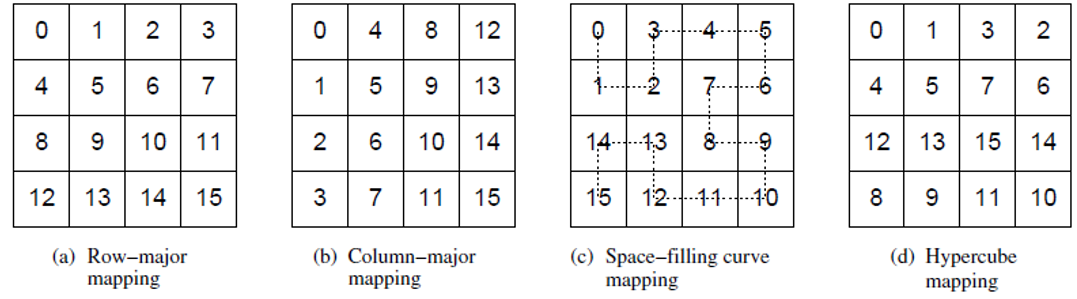
\includegraphics[width=0.7\textwidth]{figures/2-dimensional-mapping.png}
\caption{2-dimensional grid mapping}
\end{figure}

\begin{tcolorbox}[colback=red!5!white,colframe=red!75!black]
The programmer cannot explicitly specify how processes are mapped onto the processors. It is up to the MPI library to find the most appropriate mapping that reduces the cost of sending and receiving messages
\end{tcolorbox}

\hypertarget{partitioning-topologies}{%
\subsubsection{Partitioning Topologies}\label{partitioning-topologies}}

Communication operations often need to be restricted to certain subsets
of processes. MPI provides mechanisms for partitioning the group of
processes that belong to a communicator into subgroups each
corresponding to a different communicator. The simplest such mechanism
is \texttt{MPI\_Comm\_split(...)}. This operation groups processors by
color and sorts resulting groups on the key.

\begin{lstlisting}[language=C++]
int MPI_Comm_split(MPI_Comm comm, int col, int key, MPI_Comm *newComm)
\end{lstlisting}

\hypertarget{creating-cartesian-topology}{%
\subsubsection{Creating Cartesian
Topology}\label{creating-cartesian-topology}}

\begin{lstlisting}[language=C++]
int MPI_Cart_create(MPI_Comm commOld, int nDims, int *dims, int *periods, int reorder, MPI_Comm *commCart)
\end{lstlisting}

This function takes the processes in the old communicator and creates a
new communicator commCart with nDims dimensions

\begin{itemize}
\tightlist
\item
  \textbf{dims} is an array of length nDims: it specifies the size along
  each dimension of the topology
\item
  \textbf{periods} is an array of length nDims: if periods{[}i{]} is true,
  then the topology has wraparound connections along dimension i
\item
  \textbf{reorder}: determines if the processes in the new group
  (i.e.~communicator) are to be reordered or not
\end{itemize}

\hypertarget{using-cartesian-topologies}{%
\subsubsection{Using Cartesian
Topologies}\label{using-cartesian-topologies}}

\begin{itemize}
\tightlist
\item
  each process in a Cartesian topology can be identified by a vector of
  dimension nDims
\item
  since sending and receiving messages still require (one-dimensional)
  ranks, MPI provides routines to convert ranks to Cartesian coordinates

\begin{lstlisting}[language=C++]
MPI_Cart_coord(MPI_Comm commCart, int rank, int nDims, int *coords)
\end{lstlisting}

\item
  and vice-versa (coordinates to rank)

\begin{lstlisting}[language=C++]
MPI_Cart_rank(MPI_Comm commCart, int *coords, int *rank)
\end{lstlisting}
\end{itemize}

\hypertarget{collective-communication-operations}{%
\subsection{Collective Communication
Operations}\label{collective-communication-operations}}

MPI provides an extensive set of functions for performing common
collective communication operations:

\begin{itemize}
\tightlist
\item
  barrier synchronization
\item
  broadcasts: ono-to-all, all-to-all
\item
  reduction: reduce, all-reduce
\item
  prefix-sum: scan, exscan
\item
  personalized communication: gather and
\item
  scatter
\end{itemize}

each of these operations is defined over a group corresponding to the
communicator.

\clearpage